\section{Collision Avoidance} \label{sec:collision_avoidance}

% \subsection{Disturbance Repulsion}
The fundamental requirement of the proposed controller is its ability to ensure collision avoidance in the presence of external disturbances.
as the damping as proposed in \eqref{eq:control_command} does not explicitly consider external forces. Rather, the force accelerate the robot and hence results in a deviating velocity $\dot{\vecs \xi}$. Which is finally observed the controller, and corrected to approach the desired velocity $\ddot{\vecs \xi}$.\footnote{Note, that for a discrete time (digital) controller, this results in a delay.}

We further look at impact which happen during a short time period $\Delta t \ll 1$ during which a force is applied. Hence, hence we assume the velocity after impact $\vect v^I$:
\begin{align}
	 % \begin{split}
	\vect v^I
	  \approx \int_{t^I}^{t^I + \Delta t} \ddot{\vecs \xi} dt  
	  \approx \int_{t^I}^{t^I + \Delta t} \matd{M}^{-1}(\vecs \xi)  \vecs \tau_e \, dt  
	 % \end{split}
	  \label{eq:impact_velocity}
\end{align}
using the controller from \eqref{eq:robot_dynamics}, and under absence of the control force $\vecs \tau_c$ during this short timeframe. Additionally, $\{\vect \xi \}_{t^I}$ is the velocity before the impact.
 
% Since the magnitude of the normal is limited to $1$, the control weight is limited as: 
% \begin{equation}
% w(\vecs \xi) \geq \frac{\Gamma^{\mathrm{crit}} - \Gamma(\vecs \xi)}{\Gamma^{\mathrm{crit}} - 1}
% \end{equation}
% under the assumption that $\Gamma^{\mathrm{crit}} \geq 1$.

% Using the controller design from \eqref{eq:control_command} the velocity can be computed as:
% \begin{equation}
% \begin{split}
% 	\{ \vecs{\dot \xi} \}_{t} 
% 	& = \int \vecs{\ddot \xi} \, dt = \int \matd{M}^{-1} \matd{D}  \bigl( \vecs{\dot \xi} - \vecs f(\vecs \xi) \bigr) \, dt \\
% 	& = \int \matd{M}^{-1} \matd{D} \bigl( \vecs{\dot \xi} - \vecs f(\vecs \xi) \bigr) \, dt \\
% 	& = \matd{M}^{-1} \int \left( (1 - w) \matd{D}^f + w \matd{D}^{o} \right)  \bigl( \dot{\vecs \xi} - \vecs f(\vecs \xi) \bigr) dt\\
% 	& = \matd{M}^{-1} \int  \matd{D}\bigl( \vecs \xi - t \vecs f(\vecs \xi) \bigr) + C_t \\
% 	% &  \underset{}\{ {\vecs \xi} \}_0 = \vecs f(\vecs \xi) + \vecs v^I{=} \matd{M}^{-1} \matd{D}  \left( \xi - t \vecs f(\vecs \xi) \right) + C_t \\
% 	&  = \matd{M}^{-1} \matd{D}  \bigl( \vecs \xi - \{\vecs \xi\}_0  - t \vecs f(\vecs \xi) \bigr) + \vecs f(\vecs \xi) + \vecs v^I \\
%     % & \approx \int \matd{M}^{-1} \matd{D} \vect f(\vecs \xi) \, dt
% \end{split}
% \label{eq:velocity_evolution}
% \end{equation}
% using $\{ {\vecs \xi} \}_0 = \vecs f(\vecs \xi) + \vecs v^I$ to find the integration constant $C_t$.

Let us assume the desired velocity $\vect f(\vecs \xi)$ is a constant, collision free vector field which is constant and parallel to the surface to a flat surface (see Fig.~\ref{fig:disturbance_with_parallel_velocity}):
\begin{equation}
	\dotprod{\vect f(\vecs \xi)}{\vecs n(\vecs \xi)} = 0
	 \qquad
\vect f(\vecs \xi) = \text{const.}
\, , \;
\vect n(\vecs \xi) = \text{const.}
\label{eq:parallel_velocity}
\end{equation}
where $\vecs n(\vecs \xi)$ is the normal vector of the surface. 

\begin{lemma} \label{lemma:damping_collision_avoidance}
	A point like agent evolves according to the dynamical system evolves with the rigid body dynamics given in \eqref{eq:robot_dynamics} controlled by \eqref{eq:control_command}, with damping matrix $\matd{D}$ from \eqref{eq:damping_summation}, and a negligible Coriolis effect.
	A motion starting in free space remains collision-free for all times, i.e., $\Gamma( \{\vecs \xi_t\}) \geq 1$ with $t \geq 0$ if the impact velocity $v^I$ as given in \eqref{eq:impact_velocity} at time $t=0$ is limited by $\| \vect v^I\| < s^{\mathrm{f}} \| \vecs \xi - \vecs \xi^b \| / m$, with respect to the closest surface point $\vecs \xi^b \in \mathbb{R}^N$ and mass $m \in \mathbb{R}_{>0}$.
\end{lemma}

% \begin{lemma}
% 	A dynamical system evolves with the rigid body dynamics given in \eqref{eq:robot_dynamics} controlled by \eqref{eq:control_command}, with damping matrix $\matd{D}$ from \eqref{eq:damping_summation}, and a negligible Coriolis effect.
%     A point-like agent starting at position $\vect p = \{{\vecs \xi}\}_0$ close to the surface, i.e., $\Gamma( \vect p) \approx 1$ is guided by a velocity field $\vect f(\vecs \xi)$ parallel to the surface with a starting velocity $\vect v^0= \vect f(\{{\vecs \xi}\}_0)$.
%     A large disturbance towards the obstacle results in a velocity of $\{\dot{\vecs \xi}\}_0 = \vect v^I +  \vect v^0$ after the impact, with $\| \vect v^I \| \gg \| \vect v^0 \|$.
% 	A motion starting in free space remains collision-free for all times, i.e., $\Gamma( \{\vecs \xi_t\}) \geq 1$ with $t \geq 0$ if the impact velocity is limited by $\| \vect v^I\| < s^{\mathrm{o}} \| \vecs \xi - \vecs \xi^b \| / m^{\mathrm{min}}$, with respect to the closes surface point $\vecs \xi^b \in \mathbb{R}^N$ and mass $m \in \mathbb{R}_{>0}$.
% \end{lemma}

\begin{proof}

an environment where the robot should just rest, hence the desired velocity field is :
\begin{equation}
\begin{split}
	\{ \vecs{\dot \xi} \}_{T} 
	& = \int \vecs{\ddot \xi} \, dt = \int \matd{M}^{-1} \matd{D} \left( \vecs{\dot \xi} - \vect f(\vecs \xi ) \right) \, dt \\
	& = \matd{M}^{-1} \int \left( (1 - w) \matd{D}^f + w \matd{D}^{o} \right) \left( \vecs{\dot \xi} - \vect f (\vecs \xi ) \right) dt \\
	\end{split}
\label{eq:velocity_evolution}
\end{equation}

From \eqref{eq:parallel_velocity}, the vector field is constant, and the surface does not have any curvature, it follows from \eqref{eq:damping_summation} that the damping matrices $\matd{D}^o$ and $\matd{D}^f$ are constant. 
Hence, we perform the integration to find the time $T$ at which the agent stop moving towards the obstacle, which will then enable us to evaluate the distance travelled as a function of the velocity after disturbance $\vect v^I$. According to the Bony-Bezis theorem \parencite{bony1969principe}, the velocity is collision-avoiding when it is zero along the normal direction:
\begin{equation}
	\left| \vect n(\vecs \xi)^T \, \{ \vecs{\dot \xi} \}_{t} \right| = 0
\end{equation}

Thus in the following analysis, we focus on the normal component of the vectors only. Thus, in the rest of this paragraph, the component along the normal will simply be denoted by scalar values, e.g. $\xi = \dotprod{\vecs \xi}{\vecs n(\vecs \xi)} \vecs n(\vecs \xi)$.
	Furthermore, by design of the damping matrixes, we know from \eqref{eq:obstacle_damping_values} 
	that $\matd{D}^o(\vecs \xi) \vect n(\vecs \xi) = s^o \vect n(\vecs \xi)$, and from \eqref{eq:velocity_damping} we know that $\matd{D}^f(\vecs \xi) \vect n(\vecs \xi) = s^f \vect n(\vecs \xi)$. Hence, we get:
\begin{align}
	0 & = \left| \vect n(\vecs \xi)^T \, \{ \vecs{\dot \xi} \}_{t} \right| 
	  = \frac 1 m \int ( (1-w) \vect n^T \matd{D}^f \vect n + w s^{o} ) \, {\dot \xi} \, dt \nonumber \\
	   & < \frac 1 m \int  s^{f}  \, {\dot \xi} \, dt 
	   = \frac{s^f}{m} (\xi - \{ \xi \}_0 ) + v^I \, dt 
\end{align}
where $m = \max{\left(\text{eig}(\matd{M})\right)}$, we additionally assume that the damping matrices are positive definite. 

The maximum displacement follows as:
\begin{equation}
	\| {\xi} - \{\xi \}_0 \| \geq \| v^I \| {m} / {s^{\mathrm{f}}} 
\end{equation}

To see when the differences reaches zero, we can compute
\begin{equation}
 \|	\{ \vecs{\dot \xi} \}_T - \vect f(\vecs \xi) \| = 0
 \quad \Rightarrow \quad
    \| \vecs{\xi}_1 -  \vect p_1 \| = \| \vecs v^I_1 \| {m} / {s^{\mathrm{o}}} 
 \end{equation}
\end{proof}

Note, that while Lemma~\ref{lemma:damping_collision_avoidance} is under the assumption of constant desired velocity and flat surface. While most desired velocity are a function of the position, and morover obstacles are finite and hence have sume surface curvature. However, since the algorithm explores the limit, hence large disturbance forces and velocities after disturbance $\| \vect v^I \| \gg 1 \|$. As a result, the distance travelled along the surface is small, and it can be considered locally flat. Additionally, in the extreme case, the disturbance happens close to the surface, and hence the desired velocity is almost constant.  

\begin{figure}[htb]
\centering
 % \begin{subfigure}{0.99\columnwidth}
  \centerline{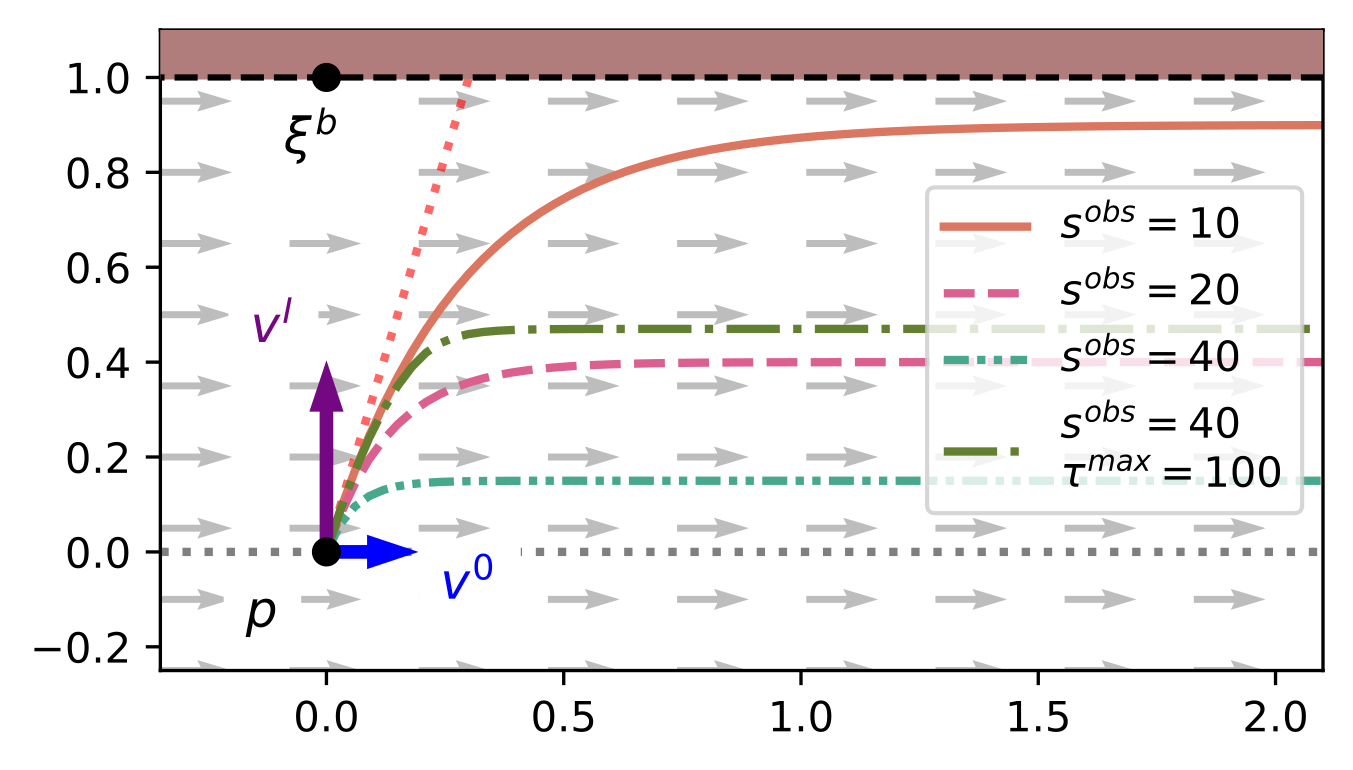
\includegraphics[width=0.99\columnwidth]{figures/parallel_avoidance_obstacle}}
  \caption{A disturbance occurs of a point-agent at position $\vect p^0$ with velocity after the impact of $\{ \dot{\vecs \xi} \}_0 = \vect v^0 + \vect v^I$. A high damping in the direction of the obstacle in the presence of a constant velocity field (gray) ensures collision avoidance. Whereas different damping values $s^{\mathrm{o}}$ and optionally a maximum repulsion force $\vecs \tau^{\mathrm{max}}$ lead to different trajectories.}
  \label{fig:disturbance_with_parallel_velocity}
% \end{subfigure}
\end{figure}
    

Note that the analysis is done for proximity regions of the obstacle. In any case, the robot enters this proximity region before a collision can occur. Hence, the proposed analysis holds as a general collision avoidance insurance.

Similarly, while we specifically analyze disturbances along the normal of the obstacle, any velocity after the disturbance can be divided into a part towards the obstacle, and a part parallel to the surface. Where a velocity parallel to the obstacle does not pose any danger for collision.
Yet, there is no guarantee against drifting into obstacles in the presence of highly curved surfaces and velocity fields. \iflong This is further discussed during the experiments in Section~\ref{sec:position_noise}, where the increased damping towards the obstacle significantly reduces collision in such scenarios. \fi

% \subsection{Disturbance Repulsion with Force Limit}
All robotic systems have a maximum force that they can exert on the environment based on the motors and their geometry, $\tau_c^{\mathrm{max}} \in \mathbb{R}_{>0}$. Additionally, such force limits are often state-dependent. A limiting force decreases the impact velocity a controller can handle while ensuring collision avoidance (Fig.~\ref{fig:disturbance_with_parallel_velocity}). Nevertheless, a maximum control force can be interpreted as adapting damping, and hence, the passivity from Theorem~\ref{theorem:passivity} holds.


